\documentclass{article}
\title{Metrics for Assessing Fund Performance}
\author{Michael Schwab \thanks }
\usepackage[margin=0.5in]{geometry}
\usepackage[utf8]{inputenc}
\usepackage{textcomp}
\usepackage{pgfplots}
\pgfplotsset{width=10cm,compat=1.9}
  
\begin{document}
    \centerline{\Large Metrics for Assessing Fund Performance}
    \section{Return}
    \begin{equation}
    return = \frac{price[end] }{price[begin]}- 1
    \end{equation}
    \section{Standard Deviation of Daily Return}
    
    \begin{equation}
        daily\_rets[i] = \frac{value[i]}{value[i-1]} -1 
    \end{equation} 
    
    \begin{equation}
        std\_metric = std(daily\_rets)
    \end{equation}
    \section{CAPM - Capital Assets Pricing Model }
     Expected Returns of an asset depends on the expected return of the market, 
    and how the asset is normally responds to the market (known as beta $\beta$) and some asset specific knowledge (alpha $\alpha$).  
    CAPM assumes $\alpha$ is unknowable, or that if it's known the efficient market hypothesis prevents all be the very fastest from taking advantage of it, it's simply zeroed out and trading is done based on the beta.  
    The quant assumes that $\alpha$ can be inferred based on additional market knowledge in ways which can be leveraged.

    $$r_i=\beta_i*r_m+\alpha_i$$

    $\alpha$ - information about a stock we can exploit (considered to be 0 by the CAPM)

    $\beta$ - positive if the stock move with the market, negative if it moves against it and 0 if there is no correlation.
    \subsection{What is Beta?}
    For the CAPM the only important factor is $\beta$. 
    
    Use linear regression to fit a line for determining $\beta$ and $\alpha$


    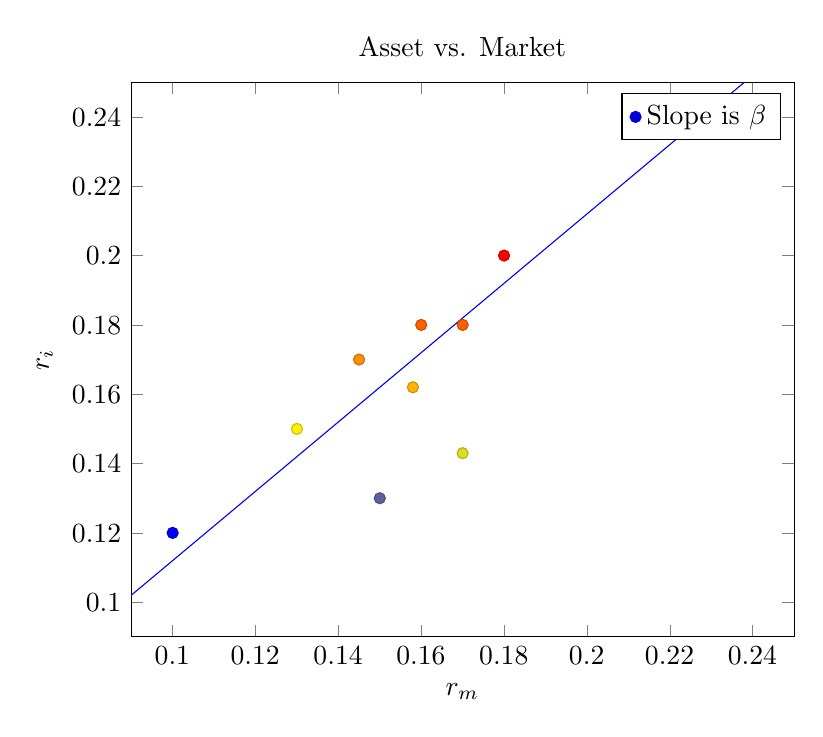
\begin{tikzpicture}
        \begin{axis}[
            title={Asset vs. Market},
            xlabel={$r_m$},
            ylabel={$r_i$},
            xmin=.09, xmax=.25,
            ymin=.09, ymax=.25 ]
        \addplot+[only marks, scatter]
        coordinates{(0.10,0.12)(0.13,0.15)(0.15,0.13)(0.145,0.17)(0.17,0.18)(.17,.143)(.16,.18)(.158,.162)(0.18,0.20)};
        \addplot[color=blue]{x + .012};
        \addlegendentry{Slope is $\beta$}
        \end{axis}
    \end{tikzpicture}

    X-axis represents what the market did, where the vertical represents what the stock did.

    Many stocks will show some kind of ellipse where the slope of the line is $\beta$

    Each stock will have it's own beta.

    $\alpha$ is the y-axis intersection.

    $\beta$ and correlation are not the same.

    Corr\_coeff (correlation coefficient), measures how far the points are from the line. 1.0 = perfect correlation, and -1.0 = perfect anti-correlation.


    \section{Portfolio Return}
    The portfolio return is the sum of the individual returns times the weight of each asset in the portfolio.
    $$r_p=\sum{w_ir_i}$$
    $r_i$ is the individual stock return
    $w_i$ is the weight of each individual stock
    Beta of the portfolio can be calculated likewise.
    $$\beta_p = \sum{w_ir_i}$$
    If we know beta and some information about a stock that could cause it to perform differently from it's beta, that's called alpha.
    

\end{document}